\begin{figure}
\centering
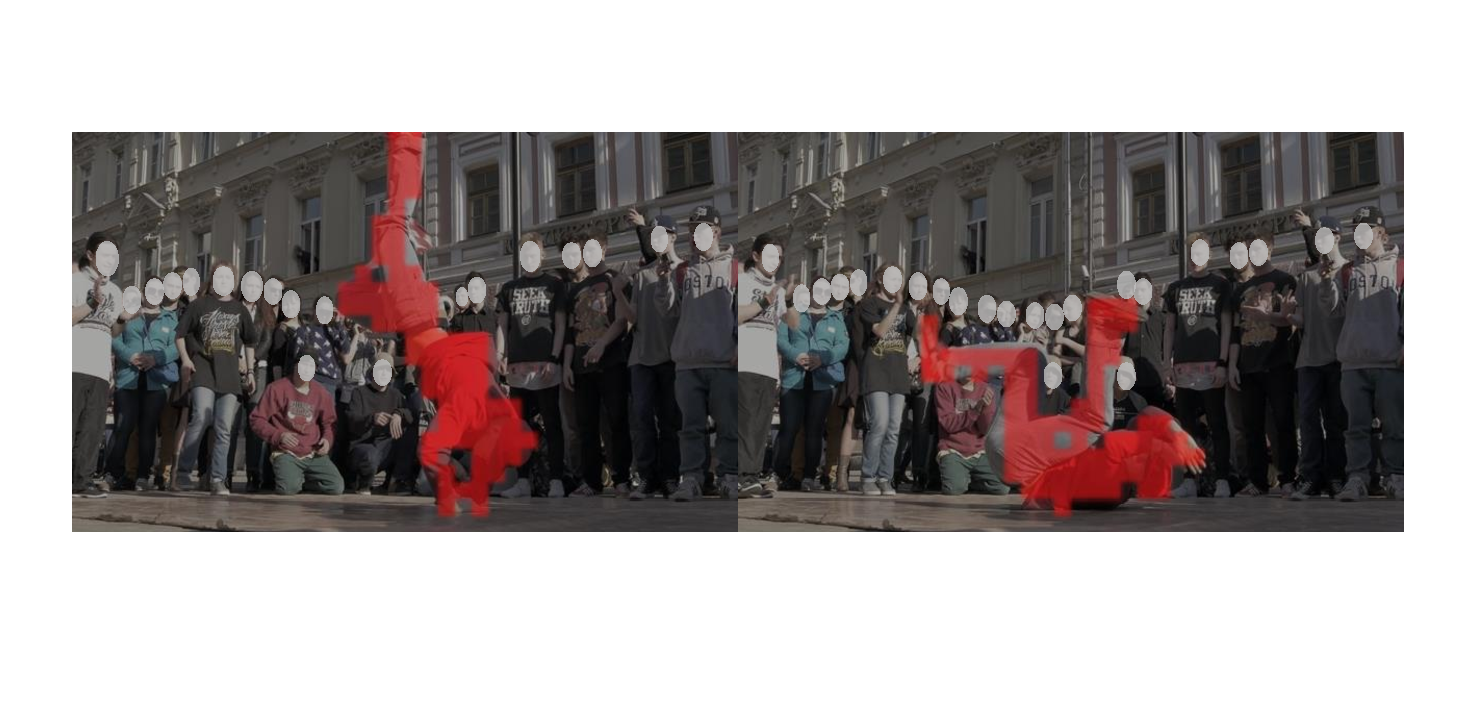
\includegraphics[width=0.95\linewidth]{figures/motion.pdf}
\caption{\textbf{Motion-Aware Representations.}
We cluster PCA-reduced intermediate image tokens by $k$-means and observe that the resulting clusters consistently separate the moving dancer from the static crowd and background, with red indicating high-response regions.
This suggests that \method learns motion-aware representations from reconstruction training, without explicit motion supervision.
}%
\label{fig:motion}
\end{figure}



